% NOLTA2025-compatible Paper Refinement
\documentclass[twocolumn,a4paper]{article} % For `dvipdfmx` user

\usepackage{nolta2025}
\usepackage{amsmath,amssymb,bbm,graphicx,subcaption,color,physics,hyperref,algorithm,algorithmic,txfonts}

\DeclareMathOperator*{\argmax}{arg\,max}
\DeclareMathOperator*{\argmin}{arg\,min}

% Custom macros
\newcommand{\inp}[2]{\left\langle {#1} \middle| {#2} \right\rangle}
\newcommand{\kb}[1]{\ket{{#1}}\!\bra{{#1}}}
\newcommand{\bbE}{\mathbb{E}} \newcommand{\bbN}{\mathbb{N}} \newcommand{\bbB}{\mathbb{B}}
\newcommand{\bbS}{\mathbb{S}} \newcommand{\bbR}{\mathbb{R}} \newcommand{\bbC}{\mathbb{C}}
\newcommand{\bbZ}{\mathbb{Z}} \newcommand{\bbH}{\mathbb{H}} \newcommand{\bbQ}{\mathbb{Q}}
\newcommand{\calX}{\mathcal{X}} \newcommand{\calY}{\mathcal{Y}} \newcommand{\calZ}{\mathcal{Z}}
\newcommand{\calH}{\mathcal{H}} \newcommand{\calV}{\mathcal{V}} \newcommand{\BSC}{\mathrm{BSC}}

% Theorem environments
\newtheorem{theorem}{Theorem}
\newtheorem{corollary}[theorem]{Corollary}
\newtheorem{lemma}[theorem]{Lemma}
\newtheorem{proposition}[theorem]{Proposition}
\newtheorem{remark}{Remark}
\newtheorem{example}{Example}
\newtheorem{definition}{Definition}
\newtheorem{conjecture}{Conjecture}
\newtheorem{postulate}{Postulate}
\newtheorem{question}{Question}
\newtheorem{observation}{Observation}

\begin{document}

\title{Quantum Annealing-Based Optimization of
Pedestrian Network Orientation:
A QUBO Formulation Study for Preventing Crowd
Crush Disasters}
\author{and Won-Joo Hwang${}^\dag$}
\address{\dag Department of Information Convergence Engineering, Pusan National University \\
Busan 46241, Republic of Korea \\
Email: \email{Cong.md@pusan.ac.kr}, \email{wjdtjsrms11@pusan.ac.kr}, \email{wjhwang@pusan.ac.kr}}
\maketitle
% \orcid{
% Mai Cong: 0009-0003-3730-8869,
% Seon-Geun Jeon: 0000-0002-5926-6642,
% Won-Joo Hwang: 0000-0001-8398-564X
% }

\abstract
Crowd crush disasters can occur when dense pedestrian flows moving in opposite directions converge within narrow urban spaces, leading to a severe loss of individual mobility and control. To address this
problem, this study proposes a quantum annealing-based orientation
optimization framework for pedestrian networks. A pedestrian network
is modeled as a weighted graph, where vertices represent intersections
and edges represent walkable paths. The objective of the optimization is to assign traffic directions to paths in order to reduce conflicts
between pedestrian flows, improve movement efficiency, and alleviate
local congestion. To this end, the framework integrates three complementary strategies: a cycle-based approach, which preserves global circulation and network connectivity; an n-hop-based approach, which reduces overall travel distance; and a flow conservation approach, which
balances inflow and outflow at each node. The final optimization problem is formulated as a Quadratic Unconstrained Binary Optimization
model and solved on the D-Wave quantum annealing platform. Experimental results show that the proposed method reduces congestion,
improves flow stability, and lowers the sum of APSP(all-pairs shortest paths), while requiring less computation time than conventional
approaches.

\endabstract
\section{Introduction} \label{sec:intro}

Crowd crush disasters are a major public safety concern and have caused severe casualties in many settings \cite{fruin1993causes}. These incidents arise not merely from high population density but from a complex interplay of factors, including environmental conditions such as topographical constraints and bottlenecks \cite{helbing2007dynamics}, as well as insufficient initial responses to fallen individuals \cite{soomaroo2012disasters}. The 2022 crowd disaster in South Korea further illustrates how extreme congestion in confined urban settings can rapidly become fatal \cite{chang2024crowd}.

Various multifaceted solutions have been explored to prevent such crowd-related accidents\cite{Nishinari2024}. However, real-world urban environments are immensely vast and complex, characterized by the simultaneous and real-time occurrence of unexpected variables such as road closures and bottlenecks. In these dynamically changing, large-scale environments, relying solely on classical computing resources presents clear limitations when attempting to account for all variables and derive optimal solutions in real time.

To overcome these challenges, this study abstracts the spatial characteristics of the target area into a graph. Building upon the foundational framework of quantum annealing\cite{Kadowaki1998}, we directly formulate the crowd control optimization problem as a Quadratic Unconstrained Binary Optimization (QUBO) model. This formulation allows us to effectively leverage quantum hardware to rapidly derive optimal paths, thereby minimizing crowd density in large-scale congestion scenarios.

The contributions of our study are summarized as follows:
\begin{itemize}
    \setlength{\itemsep}{0pt}       % 항목 간의 추가 여백 제거
    \setlength{\parsep}{0pt}        % 항목 내에서 줄바꿈 시 생기는 여백 제거
    \setlength{\parskip}{0pt}
    
    \item[(1)] Models the crowd control problem using a graph that captures complex urban networks and dynamic flows.
    \item[(2)] Proposes a novel QUBO formulation to efficiently solve large-scale routing problems via quantum annealing.
    \item[(3)] Demonstrates the viability of quantum computing for real-time disaster response through comparisons with classical algorithms.
\end{itemize}

The remainder of this paper is organized as follows. Section~\ref{sec:related} reviews related work. Section~\ref{sec:method} details proposed method. Section~\ref{sec:result} presents the simulation results, and finally, Section~\ref{sec:conclusion} concludes this paper.

\section{Related Work}
\label{sec:related}

\subsection{Crowd Safety and Pedestrian Flow Control}
\label{subsec:related_crowd}

Previous studies on crowd safety have investigated pedestrian movement using microscopic crowd simulations, evacuation models, and flow-based approaches. 
These studies have shown that dense interactions among pedestrians can reduce walking speed, generate local bottlenecks, and increase the risk of unstable crowd movement. 
In transportation and evacuation planning, contraflow strategies have also been studied to improve the utilization of road capacity by reversing selected traffic directions during emergencies~\cite{kim2008contraflow, aksu2014mathematical}. 

However, many existing approaches focus on operational crowd management or simulation-based analysis rather than the structural design of pedestrian circulation networks. 
In particular, relatively limited attention has been given to the optimization of one-way pedestrian path orientations as a preventive infrastructure-level measure.

\subsection{Graph-Based Network Orientation}
\label{subsec:related_graph}

The problem of assigning directions to the edges of an undirected graph has been extensively studied in graph theory. 
Classical results have established conditions under which an undirected graph can be oriented while preserving strong connectivity~\cite{robbins1939theorem}. 
Subsequent studies have examined strongly connected orientations, network reliability, and optimal direction assignments in transportation networks~\cite{chung1985strongly, roberts1988optimal, roberts1994optimal}. 

One-way street design has also been studied as a transportation network optimization problem. 
Existing approaches typically aim to reduce travel time, improve traffic capacity, or minimize the cost of modifying a road network~\cite{drezner1997selecting, huang2020bi, huang2020model}. 
Nevertheless, these problems become computationally challenging as the network size increases because the number of possible direction assignments grows exponentially with the number of edges. 
The complexity becomes even greater when strong connectivity, arc reversal, and multiple optimization objectives must be considered simultaneously~\cite{burkard1999minimum, bangjensen2023complexity}. 

Unlike previous studies that primarily focus on vehicle transportation, this study considers pedestrian safety-oriented network orientation. 
The proposed formulation explicitly combines local flow balance, short-path reachability, and circulation preservation.

\subsection{Quantum Annealing for Combinatorial Optimization}
\label{subsec:related_qa}

Quantum annealing has been applied to a variety of combinatorial optimization problems that can be expressed in Ising or QUBO form~\cite{qa_for_optimize}. 
Representative application domains include routing, scheduling, graph partitioning, and resource allocation. 
A QUBO model encodes binary decision variables and pairwise interactions into an energy function, allowing a quantum annealer to search for low-energy candidate solutions.

Practical execution on current quantum annealing hardware requires minor embedding, which maps logical variables and their interactions onto the limited connectivity of physical qubits~\cite{minor_embedding_inQA2, minor_embedding_inQA}. 
This embedding process may introduce additional overhead because a single logical variable can require a chain of multiple physical qubits. 
Therefore, the feasibility and quality of the embedding must be considered when designing a QA-compatible optimization model.

Building on these studies, we formulate the pedestrian network orientation problem as a QUBO model and evaluate its applicability on the D-Wave quantum annealing platform.

\section{System Model and Problem Formulation} \label{sec:model}

We consider an urban pedestrian environment represented by a weighted undirected graph $ G=(V,E,W)$, where \(V\) denotes the set of pedestrian intersections, junctions, or decision points, and \(E\) denotes the set of walkable pedestrian segments connecting them. Each undirected edge \(\{i,j\}\in E\) represents a physical pedestrian path that originally allows movement in both directions. The set \(W=\{w_{ij}\mid \{i,j\}\in E\}\) contains edge-level attributes, such as path length, effective width, walking capacity, or traversal cost. In dense pedestrian environments, bidirectional movement along narrow paths may induce counter-flow conflicts, reduce walking efficiency, and increase the risk of local congestion. The objective of this study is therefore to transform the original bidirectional pedestrian network into a directed one-way circulation network by assigning a unique walking direction to each pedestrian segment.

For each undirected edge \(\{i,j\}\in E\), an arbitrary but fixed ordering of its endpoints is imposed such that \(i<j\). We define a binary orientation variable
\begin{equation}
    x_{ij}\in\{0,1\}, \qquad \forall \{i,j\}\in E,\; i<j,
\end{equation}
where
\begin{equation}
x_{ij}=
\begin{cases}
0, & \text{if edge } \{i,j\} \text{ is oriented as } i\rightarrow j,\\
1, & \text{if edge } \{i,j\} \text{ is oriented as } j\rightarrow i.
\end{cases}
\end{equation}
The complete vector of binary orientation variables is denoted by
\begin{equation}
    \mathbf{X}
    =
    \{x_{ij}\mid \{i,j\}\in E,\; i<j\}
    \in \{0,1\}^{|E|}.
\end{equation}
The vector \(\mathbf{X}\) fully determines the directed pedestrian network $\vec{G}(\mathbf{X})=(V,\vec{E}(\mathbf{X}))$. Specifically, the directed edge set induced by \(\mathbf{X}\) is given by
\begin{equation}
\begin{aligned}
    \vec{E}(\mathbf{X})
    =
    &\{(i,j)\mid \{i,j\}\in E,\; i<j,\; x_{ij}=0\} \\
    &\cup
    \{(j,i)\mid \{i,j\}\in E,\; i<j,\; x_{ij}=1\}.
\end{aligned}
\end{equation}
Thus, each physical pedestrian segment is assigned exactly one direction. This construction eliminates direct counter-flow on individual pedestrian paths while preserving the original spatial topology of the pedestrian network.

For each node \(v\in V\), let
\begin{equation}
    \mathrm{adj}(v)=\{u\in V\mid \{u,v\}\in E\}
\end{equation}
denote the set of nodes adjacent to \(v\) in the original undirected graph. Since the binary variable \(x_{ij}\) is defined only for ordered endpoint pairs satisfying \(i<j\), the outgoing and incoming degrees of node \(v\) must distinguish between neighbors with indices greater than and smaller than \(v\). The out-degree of node \(v\) in the oriented graph \(\vec{G}(\mathbf{X})\) is defined as
\begin{equation}
    d_v^{+}(\mathbf{X})
    =
    \sum_{\substack{u\in \mathrm{adj}(v)\\v<u}}
    (1-x_{vu})
    +
    \sum_{\substack{u\in \mathrm{adj}(v)\\u<v}}
    x_{uv},
\end{equation}
where the first summation counts edges oriented from \(v\) to higher-indexed neighboring nodes, and the second summation counts edges oriented from \(v\) to lower-indexed neighboring nodes. Similarly, the in-degree of node \(v\) is
\begin{equation}
    d_v^{-}(\mathbf{X})
    =
    \sum_{\substack{u\in \mathrm{adj}(v)\\v<u}}
    x_{vu}
    +
    \sum_{\substack{u\in \mathrm{adj}(v)\\u<v}}
    (1-x_{uv}).
\end{equation}
For every node \(v\), the identity $d_v^{+}(\mathbf{X})+d_v^{-}(\mathbf{X})=|\mathrm{adj}(v)|$
holds because each incident edge is assigned exactly one direction.

A large imbalance between incoming and outgoing directions at an intersection may lead to undesirable circulation patterns. A node with many incoming directions but few outgoing directions may become a structural accumulation point, whereas a node with many outgoing directions but few incoming directions may reduce accessibility from nearby regions. To promote locally balanced circulation, we define the orientation imbalance at node \(v\) as
\begin{equation}
    B_v(\mathbf{X})
    =
    d_v^{+}(\mathbf{X})-d_v^{-}(\mathbf{X}).
\end{equation}
Substituting the definitions of \(d_v^{+}(\mathbf{X})\) and \(d_v^{-}(\mathbf{X})\), this imbalance can be written directly in terms of the binary orientation variables as
\begin{equation}
    B_v(\mathbf{X})
    =
    \sum_{\substack{u\in \mathrm{adj}(v)\\v<u}}
    (1-2x_{vu})
    +
    \sum_{\substack{u\in \mathrm{adj}(v)\\u<v}}
    (2x_{uv}-1).
\end{equation}
The local flow-balance objective is then formulated as
\begin{equation}
    F_{\mathrm{bal}}(\mathbf{X})
    =
    \sum_{v\in V}
    \left(
    B_v(\mathbf{X})
    \right)^2,
\end{equation}
or equivalently,
\begin{equation}
    F_{\mathrm{bal}}(\mathbf{X})
    =
    \sum_{v\in V}
    \left[
    \sum_{\substack{u\in \mathrm{adj}(v)\\v<u}}
    (1-2x_{vu})
    +
    \sum_{\substack{u\in \mathrm{adj}(v)\\u<v}}
    (2x_{uv}-1)
    \right]^2.
\end{equation}
Minimizing \(F_{\mathrm{bal}}(\mathbf{X})\) encourages each node to have a comparable number of incoming and outgoing pedestrian directions. Exact balance is not always attainable, especially for nodes with odd degree. Nevertheless, the squared penalty systematically discourages highly imbalanced local orientation patterns.

In addition to local balance, the oriented pedestrian network should support efficient movement between different parts of the urban space. Let \(D_{st}(\mathbf{X})\) denote the shortest directed-path distance from source node \(s\) to destination node \(t\) in \(\vec{G}(\mathbf{X})\), computed with respect to the edge weights \(w_{ij}\). If no directed path exists from \(s\) to \(t\), we set $ D_{st}(\mathbf{X})=\infty$.
Then, the total all-pairs shortest-path cost is defined as
\begin{equation}
    F_{\mathrm{dist}}(\mathbf{X})
    =
    \sum_{\substack{s,t\in V\\s\neq t}}
    D_{st}(\mathbf{X}).
\end{equation}
A smaller value of \(F_{\mathrm{dist}}(\mathbf{X})\) indicates that pedestrians can travel between node pairs with lower total directed traversal cost. This objective captures global movement efficiency, but it is meaningful only when the oriented graph preserves network-level reachability. Therefore, we require the resulting directed graph to be strongly connected, namely,
\begin{equation}
    \forall s,t\in V,\; s\neq t,
    \qquad
    \exists \text{ a directed path from } s \text{ to } t
    \text{ in } \vec{G}(\mathbf{X}).
\end{equation}

The feasible set of strongly connected orientations is therefore defined as
\begin{equation}
    \mathcal{X}_{\mathrm{sc}}
    =
    \left\{
    \mathbf{X}\in\{0,1\}^{|E|}
    \;\middle|\;
    \vec{G}(\mathbf{X}) \text{ is strongly connected}
    \right\}.
\end{equation}
This condition prevents orientation assignments that isolate regions or create unreachable destinations. It also reflects a basic structural requirement of one-way pedestrian circulation systems: despite the removal of bidirectional movement on individual paths, global accessibility should be maintained throughout the network.

Directly optimizing \(F_{\mathrm{dist}}(\mathbf{X})\) may be computationally challenging because shortest-path distances depend on the global orientation pattern of the entire graph. Therefore, a local reachability surrogate can be introduced to encourage the formation of short directed paths. To express this surrogate without introducing additional decision variables, we first define a direction-consistency function for an ordered pair of adjacent nodes \((a,b)\):
\begin{equation}
    \rho_{ab}(\mathbf{X})
    =
    \begin{cases}
    1-x_{ab}, & \text{if } a<b \text{ and } \{a,b\}\in E,\\
    x_{ba}, & \text{if } b<a \text{ and } \{a,b\}\in E.
    \end{cases}
\end{equation}
The function \(\rho_{ab}(\mathbf{X})\) is not an additional decision variable; it is only a compact expression determined entirely by the corresponding binary variable in \(\mathbf{X}\). It equals one when the oriented edge \(a\rightarrow b\) exists in \(\vec{G}(\mathbf{X})\), and zero otherwise.

Using \(\rho_{ab}(\mathbf{X})\), the number of feasible directed two-hop paths can be expressed as
\begin{equation}
    P_2(\mathbf{X})
    =
    \sum_{i\in V}
    \sum_{k\in \mathrm{adj}(i)}
    \sum_{\substack{j\in \mathrm{adj}(k)\\j\neq i}}
    \rho_{ik}(\mathbf{X})
    \rho_{kj}(\mathbf{X}).
\end{equation}
Similarly, the number of feasible directed three-hop paths is
\begin{equation}
    P_3(\mathbf{X})
    =
    \sum_{i\in V}
    \sum_{j\in \mathrm{adj}(i)}
    \sum_{\substack{k\in \mathrm{adj}(j)\\k\neq i}}
    \sum_{\substack{\ell\in \mathrm{adj}(k)\\\ell\neq j,\;\ell\neq i}}
    \rho_{ij}(\mathbf{X})
    \rho_{jk}(\mathbf{X})
    \rho_{k\ell}(\mathbf{X}).
\end{equation}
These quantities measure the extent to which the orientation supports short-range and intermediate-range directed reachability. Maximizing such short directed paths promotes locally accessible circulation structures and can serve as a structural proxy for reducing unnecessary detours. Accordingly, we define the short-path reachability objective as
\begin{equation}
    F_{\mathrm{hop}}(\mathbf{X})
    =
    -\lambda_2 P_2(\mathbf{X})
    -
    \lambda_3 P_3(\mathbf{X}),
\end{equation}
where \(\lambda_2\geq 0\) and \(\lambda_3\geq 0\) control the relative importance of two-hop and three-hop reachability. Minimizing \(F_{\mathrm{hop}}(\mathbf{X})\) is equivalent to maximizing the number of feasible short directed paths.

The pedestrian network orientation problem is then formulated as a binary constrained optimization problem. The only decision variable is the binary orientation vector \(\mathbf{X}\). Using the exact distance-based objective, the problem is written as
\begin{equation}
\begin{aligned}
    \min_{\mathbf{X}\in\{0,1\}^{|E|}}
    \quad &
    \alpha F_{\mathrm{bal}}(\mathbf{X})
    +
    \beta F_{\mathrm{dist}}(\mathbf{X})
    \\
    \mathrm{s.t.}
    \quad &
    \mathbf{X}\in\mathcal{X}_{\mathrm{sc}},
\end{aligned}
\end{equation}
where \(\alpha\geq 0\) and \(\beta\geq 0\) are weighting coefficients that control the relative importance of local balance and global movement efficiency.

\section{Proposed Method} \label{sec:method}
\begin{itemize}
    \item \textbf{Framework overview} --- Pipeline diagram: undirected $G$ $\rightarrow$ three strategy modules $\rightarrow$ combined QUBO $\rightarrow$ D-Wave $\rightarrow$ oriented $\vec{G}(\mathbf{X}^{*})$.
    \item \textbf{Cycle-based strategy} --- Short-cycle preservation as a surrogate for strong connectivity; definition of $F_{\mathrm{cyc}}(\mathbf{X})$.
    \item \textbf{$n$-hop reachability strategy} --- Reuse $F_{\mathrm{hop}}(\mathbf{X})=-\lambda_2 P_2 - \lambda_3 P_3$; justify as tractable surrogate for APSP.
    \item \textbf{Flow conservation strategy} --- Reuse $F_{\mathrm{bal}}(\mathbf{X})$; emphasize native quadratic form.
    \item \textbf{Combined QUBO} --- $H(\mathbf{X}) = \alpha F_{\mathrm{bal}} + \beta F_{\mathrm{hop}} + \gamma F_{\mathrm{cyc}}$; cubic/quartic reduction; penalty-weight selection.
    \item \textbf{Solving on D-Wave} --- Minor embedding, chain strength, number of reads, post-processing.
    \item \textbf{Algorithm summary} --- Pseudocode for the full pipeline.
\end{itemize}

\section{Simulation Results} \label{sec:result}
Present all of the results that you got, compare with classical algorithm here
\section{Conclusion} \label{sec:conclusion}



\bibliographystyle{plain}
\bibliography{Fig_MaiDinhCong/ref}

\end{document}




% %\documentclass[twocolumn,a4paper,dvipdfmx,reprint,amsmath,amssymb,aps,superscriptaddress,showkeys]{article} %<--- For `dvipdfmx' user
% % \documentclass[twocolumn,a4paper]{article} %<--- For `pdflatex`' user
% \documentclass[reprint,amsmath,amssymb,aps,superscriptaddress,showkeys]{revtex4-2}
% \usepackage{nolta2025}
% \usepackage{amsmath} %<--- Please uncomment this command if you use amsmath package.
% \usepackage{graphicx}
% \usepackage{bbm}
% \usepackage{subcaption}
% \usepackage{color}
% \usepackage{physics}
% \usepackage{hyperref}
% \usepackage{algorithm}
% \usepackage{algorithmic}
% \DeclareMathOperator*{\argmax}{arg\,max}
% \DeclareMathOperator*{\argmin}{arg\,min}
% \newcommand{\inp}[2]{\left\langle {#1} \middle| {#2} \right\rangle}
% \newcommand{\kb}[1]{\ket{{#1}}\!\bra{{#1}}}
% \newcommand{\bbE}{\mathbb{E}}
% \newcommand{\bbN}{\mathbb{N}}
% \newcommand{\bbB}{\mathbb{B}}
% \newcommand{\bbS}{\mathbb{S}}
% \newcommand{\bbR}{\mathbb{R}}
% \newcommand{\bbC}{\mathbb{C}}
% \newcommand{\bbZ}{\mathbb{Z}}
% \newcommand{\bbH}{\mathbb{H}}
% \newcommand{\bbQ}{\mathbb{Q}}
% \newcommand{\calX}{\mathcal{X}}
% \newcommand{\calY}{\mathcal{Y}}
% \newcommand{\calZ}{\mathcal{Z}}
% \newcommand{\calH}{\mathcal{H}}
% \newcommand{\calV}{\mathcal{V}}
% \newcommand{\BSC}{\mathrm{BSC}}
% \newtheorem{theorem}{Theorem}
% \newtheorem{corollary}[theorem]{Corollary}
% \newtheorem{lemma}[theorem]{Lemma}
% \newtheorem{proposition}[theorem]{Proposition}
% \newtheorem{remark}{Remark}
% \newtheorem{example}{Example}
% \newtheorem{definition}{Definition}
% \newtheorem{conjecture}{Conjecture}
% \newtheorem{postulate}{Postulate}
% \newtheorem{question}{Question}
% \newtheorem{observation}{Observation}
% \usepackage{txfonts}
% \usepackage{color}
% \usepackage{algorithm}
% \usepackage{algorithmic}
% \begin{document}
% \bibliographystyle{plain}  % or apa, ieeetr, etc.
% \bibliography{Fig_MaiDinhCong/ref}
% \title{Fault-Tolerant Minor Embedding in Quantum Annealers}

% \author{
%   Mai Dinh Cong, Seon-Geun Jeon, Won-Joo Hwang
% }
% \address{
% \dag Department of Information Convergence Engineering, Pusan National University \\
% Busan, 46241, Republic of Korea \\
% Email: \email{Cong.md@pusan.ac}, \email{wjdtjsrms11@pusan.ac.kr}, \email{wjhwang@pusan.ac.kr}
% }

% \maketitle

% %%% Notice for ORCiD:
% % Do not destroy the format, e.g., do not remove/replace the colons, spaces, or commas.
% % Though do not hesitate to add another record following the form.
% \orcid{
% First Author: 0009-0003-3730-8869,
% Second Author: 0000-0002-5926-6642,
% Third Author: 0000-0001-8398-564X
% }

% \abstract
% Quantum annealing (QA) is a specialized quantum computing technique designed to solve combinatorial optimization problems by exploiting quantum tunneling and superposition. However, its performance is constrained by hardware limitations that require minor embedding. This embedding process introduces errors through broken chains and thermal noise. We develop a fault-tolerant minor embedding method that substantially enhances solution accuracy on D-Wave quantum annealers. Experimental results validate our approach's effectiveness in mitigating errors and advancing practical quantum optimization.
% \endabstract
% \section{Introduction}
% Quantum annealing (QA)~\cite{qa_for_optimize} is a specialized computational paradigm that leverages quantum mechanical principles such as tunneling and superposition to solve combinatorial optimization problems. The process begins with the system initialized in the ground state of a known initial Hamiltonian and gradually evolves toward the ground state of a problem-specific Hamiltonian~\cite{schrodinger_equation}. If the evolution is sufficiently slow, the adiabatic theorem guarantees that the system remains in its ground state throughout the process, ideally reaching the global optimum at the end of the annealing schedule. This method has shown strong potential for solving optimization tasks that are computationally intractable for classical algorithms.

% A major challenge in deploying QA on actual hardware lies in the problem of \textit{minor embedding}~\cite{minor_embedding_inQA}, which involves mapping a logical problem graph often with arbitrary connectivity onto the sparse and constrained topology of physical qubits in a quantum annealer. This process requires each logical variable to be assigned to a chain of physical qubits, with couplings between logical variables preserved by available hardware connections. As problem size and connectivity increase, constructing embeddings that are both valid and efficient becomes increasingly difficult, especially in the presence of defective or unreliable qubits. Since embedding quality directly influences performance, scalability, and solution reliability, it is a key concern in the design of practical quantum annealing workflows.

% In addition to embedding constraints, quantum annealers are subject to various sources of error, including thermal noise, decoherence, and hardware imperfections. These factors can cause the system to deviate from its ideal evolution, leading to erroneous or suboptimal solutions. Quantum Error Correction (QEC)~\cite{QEC_cong} provides a theoretical framework for combating such noise by encoding logical qubits into multiple physical qubits and enabling error detection and correction. However, the high overhead and analog nature of QA make QEC impractical for current generation annealers~\cite{limited_QEC_QA}.

% To address these limitations, Quantum Error Mitigation (QEM)~\cite{RevModPhys.95.045005} has emerged as a viable alternative. Unlike QEC, QEM does not require additional qubits or redundant encoding. Instead, it applies algorithmic techniques to infer error free results from noisy quantum computations. One notable example is Zero-Noise Extrapolation (ZNE)~\cite{ZNE_QAM}, which estimates ideal observables by analyzing outputs under varying levels of artificial noise. While ZNE has shown success across multiple quantum platforms, its use in QA is still limited by implementation constraints.

% Another strategy specific to QA is Quantum Annealing Correction (QAC)~\cite{QAC_minor_embedding}, which employs repetition codes and ferromagnetic penalties to suppress errors during the annealing process. Although QAC can improve robustness, it also increases resource consumption and embedding complexity. In contrast, QEM techniques such as ZNE are more resource-efficient and are especially beneficial when integrated with robust embedding mechanisms and post-processing methods.

% This paper investigates fault-tolerant strategies for minor embedding in quantum annealing systems affected by hardware faults. We propose a risk-aware embedding algorithm that incorporates local penalty models to avoid unreliable qubits and minimize chain break probability. By combining embedding robustness with lightweight error mitigation principles, our method improves the quality and feasibility of QA solutions in noisy and resource constrained environments. Through theoretical modeling and experimental validation on D-Wave Advantage hardware using synthetic Ising instances, we demonstrate that our approach enhances embedding success rate and solution reliability, offering a practical path forward for scalable quantum annealing applications.
% We consider a quantum annealing system based on the Pegasus hardware graph, in which embedding a logical optimization problem into the physical architecture is complicated by the presence of faulty components. The model consists of the following elements:
% \section{Model Definition}
% \begin{itemize}
%     \item A \textbf{logical graph} $\tilde{G} = (\tilde{V}, \tilde{E})$, where nodes represent logical variables and edges represent logical couplings;
    
%     \item A \textbf{physical hardware graph} $G = (V, E)$, representing the Pegasus qubit topology;

%     \item Sets of \textbf{faulty components}, $V_{\text{faulty}} \subseteq V$ and $E_{\text{faulty}} \subseteq E$, representing defective qubits and couplers;

%     \item A mapping from each logical qubit $\tilde{i} \in \tilde{V}$ to a connected subset $\mathcal{C}_{\tilde{i}} \subseteq V \setminus V_{\text{faulty}}$ (a chain);

%     \item A condition ensuring each logical interaction $(\tilde{i}, \tilde{j}) \in \tilde{E}$ is supported by a physical coupler $(u, v) \in E \setminus E_{\text{faulty}}$ with $u \in \mathcal{C}_{\tilde{i}}$, $v \in \mathcal{C}_{\tilde{j}}$.
% \end{itemize}

% To encourage stable chains, strong ferromagnetic couplings $\gamma > 0$ are applied within each chain. Additionally, we define a \textbf{risk penalty function} $r: V \to \mathbb{R}_{\geq 0}$ to disincentivize the use of qubits that are spatially close to faults:
% \begin{equation}
% r(v) = \sum_{u \in V_{\text{faulty}}} \frac{1}{1 + \mathrm{dist}_G(v, u)},
% \label{eq:risk_function}
% \end{equation}
% where $\mathrm{dist}_G(v, u)$ is the shortest-path distance in the original hardware graph.

% \subsection{Fault-Tolerant Embeddability}

% A robust embedding should be compact, avoid faulty regions, and minimize the probability of chain breaks. To capture these design goals, we define a total embedding cost based on three competing factors:

% \begin{enumerate}
%     \item \textbf{Chain size}: the total number of physical qubits used;
%     \item \textbf{Risk exposure}: penalizes chains that include qubits near faults;
%     \item \textbf{Chain break probability}: modeled as a decreasing function of $\gamma$.
% \end{enumerate}

% We formulate the minor embedding task as a constrained optimization problem. Let ${\mathcal{C}{\tilde{i}}}$ be a collection of chains, where each chain $\mathcal{C}{\tilde{i}}$ corresponds to a logical qubit $\tilde{i} \in \tilde{V}$, and let $\gamma > 0$ denote the intra-chain ferromagnetic coupling strength. The objective is to minimize the total embedding cost, defined as:

% \begin{equation}
% \min_{{\mathcal{C}{\tilde{i}}},\ \gamma > 0} \left(
% \sum{\tilde{i} \in \tilde{V}} \sum_{v \in \mathcal{C}{\tilde{i}}} \left[ 1 + \lambda \cdot r(v) \right]
% + \mu \cdot P{\text{break}}(\gamma)
% \right),
% \label{eq:objective}
% \end{equation}

% where $\lambda > 0$ is a regularization parameter controlling the trade-off between chain size and proximity to faulty regions (as quantified by the risk function $r(v)$), and $\mu > 0$ weighs the importance of chain robustness. The chain break probability is modeled as $P_{\text{break}}(\gamma) = e^{-\beta \gamma} + \epsilon_{\text{noise}}$, where $\beta$ is a physical parameter associated with thermal noise, and $\epsilon_{\text{noise}}$ captures residual hardware-level noise.

% The optimization is subject to the following constraints: each chain $\mathcal{C}{\tilde{i}}$ must induce a connected subgraph within the physical hardware graph, and chains assigned to distinct logical qubits must be disjoint, i.e., $\mathcal{C}{\tilde{i}} \cap \mathcal{C}{\tilde{j}} = \emptyset$ for all $\tilde{i} \ne \tilde{j}$. Furthermore, the chains must exclude faulty qubits, implying $\mathcal{C}{\tilde{i}} \subseteq V \setminus V_{\text{faulty}}$ for all $\tilde{i}$. Each logical coupling $(\tilde{i}, \tilde{j}) \in \tilde{E}$ must be physically realizable by ensuring that there exists at least one functional physical coupler $(u, v) \in E \setminus E_{\text{faulty}}$ such that $u \in \mathcal{C}{\tilde{i}}$ and $v \in \mathcal{C}{\tilde{j}}$. Lastly, the intra-chain coupling strength must be sufficiently large to ensure alignment within chains, i.e., $\gamma \gg |\tilde{J}_{\tilde{i}\tilde{j}}|$ for all logical couplings.

% This formulation yields a fault aware, resource efficient, and hardware compatible minor embedding strategy suitable for real world quantum annealers like D-Wave Advantage.
% \section{Fault-Tolerant Minor Embedding Algorithm}

% This section presents a detailed theoretical analysis of a fault-tolerant minor embedding algorithm specifically designed for Pegasus-based quantum annealers, analogous in approach to the Minorminer algorithm commonly utilized within the D-Wave quantum annealing framework. The primary objective of this embedding algorithm is to construct an embedding that minimizes both the physical qubit usage and the chain break probability, thereby enhancing the robustness and fidelity of quantum annealing solutions.

% The proposed algorithm begins by taking as input a logical graph $\tilde{G} = (\tilde{V}, \tilde{E})$ representing the optimization problem, along with the physical Pegasus hardware graph $G = (V, E)$, which includes sets of faulty qubits $V_{\text{faulty}}$ and faulty couplers $E_{\text{faulty}}$. The initial parameters set include penalty coupling strength $\gamma$, balance factor $\mu$, and parameters governing the chain break probability, denoted by $\beta$ and $\epsilon_{\text{noise}}$.

% \subsection{Algorithmic Framework}

% To realize the embedding formulation introduced in Section~3, we propose a practical, heuristic-based algorithm that incorporates hardware fault awareness and localized risk sensitivity into the minor embedding process. The key innovation lies in extending traditional embedding routines, such as those used in \texttt{minorminer} by incorporating a qubit level penalty function that disincentivizes the use of qubits near faulty regions.

% \subsubsection*{Overview}

% The embedding problem is computationally intractable in general; it is NP-complete to even determine the existence of a valid embedding. Therefore, heuristic methods are typically employed in practice. Our proposed algorithm, \textit{Risk-Aware Minor Embedding} (RAME), retains the greedy, iterative spirit of classical methods while introducing a principled mechanism to favor structurally reliable subregions of the hardware.

% Given a logical problem graph $\tilde{G} = (\tilde{V}, \tilde{E})$ and a physical Pegasus graph $G = (V, E)$ with known faulty components $(V_{\text{faulty}}, E_{\text{faulty}})$, the RAME algorithm proceeds through the following stages:

% \subsubsection*{Stage 1: Fault-Aware Preprocessing}

% The first stage involves constructing a fault-aware subgraph $G' = (V', E')$ derived from the original hardware graph $G = (V, E)$. This is done by explicitly removing all known faulty qubits and couplers, as identified by the sets $V_{\text{faulty}}$ and $E_{\text{faulty}}$, respectively. Formally:

% \begin{align*}
% V' &= V \setminus V_{\text{faulty}}, \\
% E' &= E \setminus E_{\text{faulty}}.
% \end{align*}

% This preprocessing step is critical, as attempting to embed logical variables using defective components would lead to unreliable computation or complete failure during quantum annealing execution. By ensuring that all chains are constructed solely from the fault-free subgraph $G'$, the algorithm guarantees that subsequent embedding operations are constrained to feasible and operational regions of the hardware.

% In practice, this stage may also incorporate up-to-date hardware diagnostics provided by the quantum annealing system, allowing the embedding algorithm to dynamically adapt to the evolving fault landscape of the processor. The output of this step is a clean, functional graph over which chain construction and optimization are performed.

% \subsubsection*{Stage 2: Risk Score Computation}

% Even after excluding known faulty components, qubits in close proximity to defective regions may still be at elevated risk of failure due to hardware cross-talk, calibration instability, or thermal effects. To account for this, we compute a quantitative \textit{risk score} for each remaining qubit $v \in V'$, defined as:

% \begin{equation}
% r(v) = \sum_{u \in V_{\text{faulty}}} \frac{1}{1 + \mathrm{dist}_G(v, u)},
% \label{eq:risk_repeat}
% \end{equation}

% where $\mathrm{dist}_G(v, u)$ denotes the shortest-path distance from $v$ to each faulty qubit $u$ in the original hardware graph $G$ (before fault removal). This formulation ensures that qubits closer to faulty regions are assigned higher risk scores, with the influence of each fault decaying inversely with distance.

% This approach provides a smooth, differentiable estimate of reliability across the hardware graph, rather than relying on binary fault status alone. To optimize efficiency, these scores are computed once and cached for reuse in downstream stages. The result is a scalar risk profile over $V'$, informing the algorithm about spatial reliability variations in the hardware.

% \subsubsection*{Stage 3: Penalty Weight Assignment}

% To guide the embedding algorithm away from unreliable regions, we introduce a penalty-weight function $w: V' \rightarrow \mathbb{R}_{\geq 1}$, which assigns a soft cost to each qubit based on its previously computed risk score. The penalty weight is defined as:

% \begin{equation}
% w(v) = 1 + \lambda \cdot r(v),
% \end{equation}

% where $\lambda > 0$ is a hyperparameter that controls the sensitivity of the algorithm to hardware risk. When $\lambda = 0$, the algorithm ignores risk entirely and behaves like a conventional embedding routine. As $\lambda$ increases, the algorithm becomes more conservative, actively avoiding qubits near faults even if they are otherwise usable.

% Importantly, these weights are not treated as hard constraints; rather, they influence the cost function minimized during chain selection. In this way, the algorithm can still use higher-risk qubits if no better options exist, but it will naturally favor low-risk regions when constructing chains. This allows for a principled balance between robustness and resource utilization, especially in hardware-limited scenarios.

% \subsubsection*{Stage 4: Guided Chain Construction}

% The core embedding process follows a greedy, iterative strategy where logical variables are embedded one by one. For each logical qubit $\tilde{i} \in \tilde{V}$, the algorithm selects a connected subset $\mathcal{C}_{\tilde{i}} \subseteq V'$ such that:

% \begin{enumerate}
%     \item $\mathcal{C}_{\tilde{i}}$ minimizes the cumulative penalty $\sum_{v \in \mathcal{C}_{\tilde{i}}} w(v)$;
%     \item $\mathcal{C}_{\tilde{i}}$ satisfies the connectivity requirement;
%     \item $\mathcal{C}_{\tilde{i}}$ is disjoint from all previously assigned chains $\mathcal{C}_{\tilde{j}}$ for $\tilde{j} < \tilde{i}$.
% \end{enumerate}

% This process can be implemented by search procedures over the weighted graph $G'$, where node traversal costs are given by $w(v)$. If no suitable embedding for $\tilde{i}$ is found due to resource exhaustion or connectivity failures, the algorithm either backtracks or restarts with a different random order of logical variables.

% \subsubsection*{Stage 5: Logical Edge Realization}

% After all logical qubits are assigned to chains, the algorithm verifies that the embedding respects the logical graph structure. Specifically, for each logical edge $(\tilde{i}, \tilde{j}) \in \tilde{E}$, there must exist at least one physical edge $(u, v) \in E'$ such that $u \in \mathcal{C}_{\tilde{i}}$ and $v \in \mathcal{C}_{\tilde{j}}$. This ensures that the intended logical coupling can be realized using available hardware connections.

% If such an edge is not found, the algorithm attempts to locally expand one or both chains to establish the necessary connection. If this still fails e.g., due to faulty qubits or routing conflicts the entire embedding process may be restarted. This validation is essential to ensure that the physical Hamiltonian faithfully represents the original logical problem.


% \subsubsection*{Stage 6: Robustness Optimization}

% As a final optional step, the algorithm adjusts the intra chain ferromagnetic coupling strength $\gamma$ to improve the reliability of the embedded solution. To ensure that chains behave as single logical units, the coupling must be significantly stronger than any logical interaction:

% \[
% \gamma \gg \max_{(\tilde{i}, \tilde{j}) \in \tilde{E}} |\tilde{J}_{\tilde{i}\tilde{j}}|.
% \]

% Choosing an appropriate value for $\gamma$ is crucial: if it is too small, chains are more likely to break due to thermal fluctuations or noise; if it is too large, it can dominate the energy landscape and distort the problem’s solution space. In practice, $\gamma$ is either selected empirically or computed using analytical bounds based on the instance and hardware constraints.

% This stage enhances the robustness of the embedding, particularly under noisy or imperfect hardware conditions, and plays a key role in achieving high-quality solutions in practical quantum annealing applications.

% \subsubsection*{Algorithm Summary}

% The complete \textit{Risk-Aware Minor Embedding} procedure is summarized in Algorithm~\ref{alg:rame}.

% \begin{algorithm}[H]
% \caption{Risk-Aware Minor Embedding (RAME)}
% \label{alg:rame}
% \begin{algorithmic}[1]
% \REQUIRE Logical graph $\tilde{G} = (\tilde{V}, \tilde{E})$, physical hardware graph $G = (V, E)$, sets of faulty qubits $V_{\text{faulty}}$ and faulty couplers $E_{\text{faulty}}$, risk sensitivity parameter $\lambda > 0$
% \ENSURE Embedding $\{\mathcal{C}_{\tilde{i}}\}_{\tilde{i} \in \tilde{V}}$ or failure
% \vspace{0.1cm}
% \STATE \textbf{Construct Fault-Aware Subgraph:}
% \STATE \quad $V' \gets V \setminus V_{\text{faulty}}$
% \STATE \quad $E' \gets E \setminus E_{\text{faulty}}$

% \STATE \textbf{Compute Risk Scores:}
% \FOR{each $v \in V'$}
%     \STATE $r(v) \gets \sum_{u \in V_{\text{faulty}}} \frac{1}{1 + \mathrm{dist}_G(v, u)}$
% \ENDFOR

% \STATE \textbf{Assign Penalty Weights:}
% \FOR{each $v \in V'$}
%     \STATE $w(v) \gets 1 + \lambda \cdot r(v)$
% \ENDFOR

% \STATE Initialize empty embedding: $\mathcal{C}_{\tilde{i}} \gets \emptyset$ for all $\tilde{i} \in \tilde{V}$

% \STATE \textbf{Embed Logical Qubits Iteratively:}
% \FOR{each $\tilde{i} \in \tilde{V}$ (in random order)}
%     \STATE Find a connected subgraph $\mathcal{C}_{\tilde{i}} \subseteq V'$ minimizing $\sum_{v \in \mathcal{C}_{\tilde{i}}} w(v)$
%     \STATE Ensure $\mathcal{C}_{\tilde{i}}$ is disjoint from all previously assigned chains
%     \IF{no such chain can be constructed}
%         \STATE \textbf{Restart} with a new ordering or backtrack
%     \ENDIF
% \ENDFOR

% \STATE \textbf{Validate Logical Edges:}
% \FOR{each $(\tilde{i}, \tilde{j}) \in \tilde{E}$}
%     \IF{no $(u, v) \in E'$ such that $u \in \mathcal{C}_{\tilde{i}}$, $v \in \mathcal{C}_{\tilde{j}}$}
%         \STATE Attempt to expand $\mathcal{C}_{\tilde{i}}$ or $\mathcal{C}_{\tilde{j}}$ locally
%         \IF{no valid edge can be established}
%             \STATE \textbf{Restart} embedding process
%         \ENDIF
%     \ENDIF
% \ENDFOR

% \RETURN $\{\mathcal{C}_{\tilde{i}}\}_{\tilde{i} \in \tilde{V}}$
% \end{algorithmic}
% \end{algorithm}
% \section{The result}
% \subsection{Experimental Setup}
% \label{sec:experimental-setup}

% \subsubsection{Instance Generation}

% To evaluate the performance of the proposed risk-aware embedding strategy, we designed a series of experiments involving synthetically generated Ising problems. Three experiments were conducted to address concerning the robustness of embedding algorithms under fault-aware constraints. Each experimental instance consists of an Ising Hamiltonian defined on a randomly generated logical graph $\tilde{G} = (\tilde{V}, \tilde{E})$, with numerical parameters assigned to both node biases and pairwise couplings.

% The generation of each Ising instance follows a two-step procedure:

% \begin{enumerate}
%     \item \textbf{Random Graph Construction.} The logical graph $\tilde{G}$ is synthesized using the Erdős–Rényi (ER) random graph model. For each instance, a graph is generated with a fixed number of logical qubits $|\tilde{V}| = n$ and a tunable edge density parameter $p \in [0, 1]$, where each possible edge between pairs of nodes is included independently with probability $p$. The ER model was selected for its statistical uniformity and its capacity to simulate a wide range of connectivity patterns without introducing topological bias.
    
%     \item \textbf{Parameter Assignment.} After the graph topology is fixed, numerical values are assigned to the Ising Hamiltonian terms. Specifically, for each node $\tilde{i} \in \tilde{V}$, a bias $h_{\tilde{i}}$ is drawn uniformly at random from the interval $[-1, +1]$, and for each edge $(\tilde{i}, \tilde{j}) \in \tilde{E}$, a coupling strength $J_{\tilde{i}\tilde{j}}$ is likewise sampled from $[-1, +1]$. This uniform sampling prevents pathological or degenerate cases that could bias the experimental evaluation.
% \end{enumerate}

% % Note that for the experiment addressing RQ2—focused specifically on the structural feasibility and quality of minor embeddings—the resolution of the Ising problem is not necessary. In that case, only the graph generation phase is required.

% \subsubsection{Quantum Annealing Infrastructure}

% All Ising instances were solved on a D-Wave Advantage 4.1 quantum annealer. This system represents the latest generation of commercially available quantum annealing processors at the time of writing and offers significant improvements in hardware scale and reliability.

% The Advantage 4.1 processor features:
% \begin{itemize}
%     \item A total of $5627$ physical qubits,
%     \item A connectivity architecture based on the Pegasus topology,
%     \item Hardware-level support for programmable biases and couplings,
%     \item An improved qubit yield, with the lowest rate of broken qubits among D-Wave devices currently in operation.
% \end{itemize}


% \subsubsection{Fault Simulation and Embedding Environment}

% To ensure consistency between simulations and physical execution, we replicate hardware fault behavior in software for both embedding and evaluation. Faulty qubits and couplers are simulated by removing a subset of physical nodes and edges from the Pegasus graph used in embedding.

% In alignment with reported hardware statistics, we assume a fault rate of $10\%$ for qubits, and simulate this by randomly removing $10\%$ of the nodes in the Pegasus graph prior to embedding. This simulates realistic operating conditions of the annealer while allowing reproducibility and controlled experimentation in software environments.

% For embedding, we use both a standard baseline embedding algorithm (\texttt{minorminer}) and our proposed \textit{Risk-Aware Minor Embedding} (RAME) strategy. Both embedding algorithms operate on the same set of generated problem instances and hardware configurations, enabling controlled comparisons in both embedding quality and quantum annealing performance.
% \subsection{Performance Evaluation}
% % \begin{figure}[t]
% % 	\centering
% % 	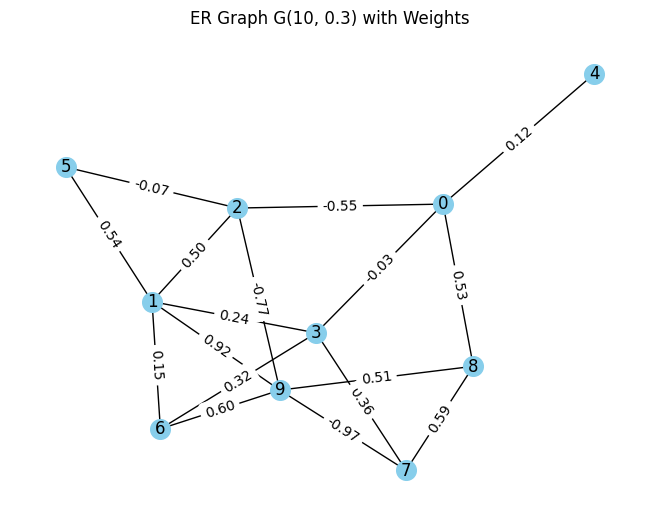
\includegraphics[width=\linewidth]{Fig_MaiDinhCong/logical problem}
% % 	\caption{An example of a logical problem consisting of 10 logical qubits, with an edge creation density of 0.3.}
% % 	\label{fig:logical_problem}
% % 	\vspace{-0.25cm}
% % \end{figure}

% \begin{figure}[t]
% 	\centering
% 	\begin{minipage}[t]{0.24\textwidth}
% 	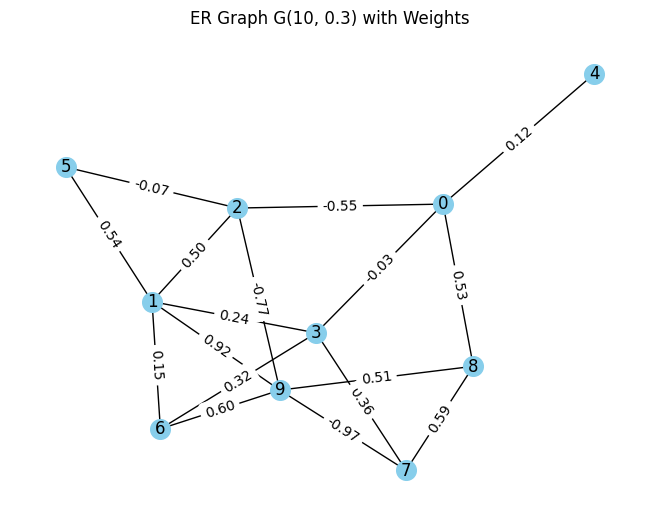
\includegraphics[ width=\linewidth]{Fig_MaiDinhCong/logical problem}
% 		\subcaption{}
% 	\end{minipage}
% 	\begin{minipage}[t]{0.24\textwidth}
% 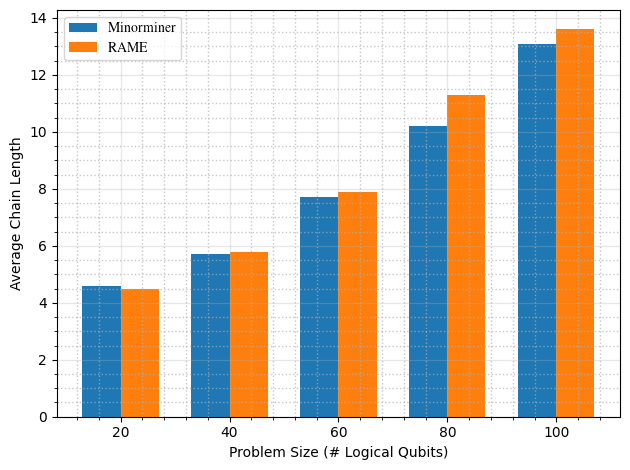
\includegraphics[ width=\linewidth]{Fig_MaiDinhCong/rame vs minor.png}
% 		\subcaption{}
% 	\end{minipage}
% 	\caption{The left figure shows An example of a logical problem consisting of 10 logical qubits, with an edge creation density of 0.3 and the right figure show average chain length (ACL) of logical qubits after performing minor embedding, as the problem size increases from 40 to 100. The results are compared against the Minorminer baseline. The edge density of the problem graphs is fixed at 0.5.}
% 	\label{fig:average and percent}
% \end{figure}

% Figure~\ref{fig:logical_problem} illustrates a simple instance of a logical Ising problem consisting of 10 logical qubits. The problem is generated with an edge creation density of 30\%, meaning that each pair of logical qubits has a 30\% chance of being connected by an interaction. Our objective is to embed this logical problem (the source graph) into the target hardware graph, which represents a Pegasus topology containing approximately 5627 physical qubits, with 10\% of them randomly marked as faulty. A valid embedding must ensure that each logical qubit is represented by a connected set of physical qubits (a chain), and that for every edge in the logical graph, there exists at least one functional physical edge connecting the two corresponding chains in the target graph.



% % \begin{figure}[t]
% % 	\centering
% % 	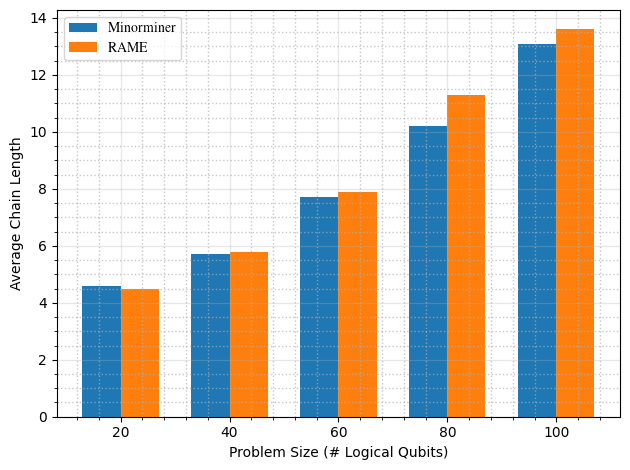
\includegraphics[width=3.2in]{Fig_MaiDinhCong/rame vs minor.png}
% % 	\caption{Average chain length (ACL) of logical qubits after performing minor embedding, as the problem size increases from 40 to 100. The results are compared against the Minorminer baseline. The edge density of the problem graphs is fixed at 0.5.}
% % 	\label{fig:ACL}
% % 	\vspace{-0.25cm}
% % \end{figure}
% Figure~\ref{fig:ACL} illustrates the trend in average chain length (ACL) as a function of problem size, with the number of logical qubits increasing from 20 to 100. All problem instances are generated using Erdős–Rényi random graphs with a fixed edge density of 0.5. The figure compares the performance of our proposed fault-aware embedding method against the standard \texttt{minorminer} baseline. As the number of logical variables increases, the connectivity of the problem graph grows, resulting in denser interactions. For instance, at 20 logical qubits, the ACL is 4.5, whereas it increases to 13.2 at 100 logical qubits. This growth occurs because embedding such graphs onto quantum hardware requires each logical qubit to be mapped to a chain of connected physical qubits. To preserve the original couplings between logical qubits, the embedding must ensure that their corresponding chains remain physically adjacent and connected via hardware couplers. However, as the problem size and connectivity increase, satisfying these constraints necessitates longer chains to maintain the required physical connectivity. This increase in chain length stems from the limited native connectivity of the Pegasus hardware graph, which becomes increasingly strained as the logical problem scales. While longer chains are necessary, they also introduce higher risks of chain breaks and greater physical qubit overhead. This motivates the need for embedding strategies that effectively balance chain compactness and robustness. Our results demonstrate that the proposed method achieves competitive performance compared to \texttt{minorminer}, the standard embedding algorithm used by D-Wave systems. For example, at 100 logical qubits, our method yields an ACL of 13.7, while \texttt{minorminer} produces an ACL of 13.2. However, unlike our fault-aware approach, \texttt{minorminer} does not account for potential broken qubits, which may compromise solution reliability in practical deployments.

% \begin{figure}[t]
% 	\centering
% 	\begin{minipage}[t]{0.24\textwidth}
% 	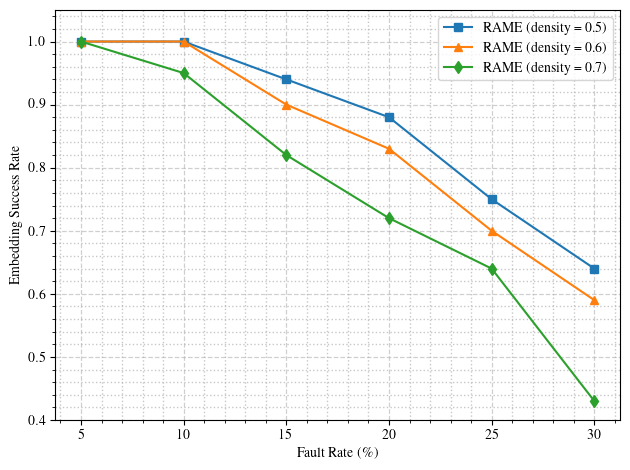
\includegraphics[ width=\linewidth]{Fig_MaiDinhCong/embedding successful rate.png}
% 		\subcaption{}
% 	\end{minipage}
% 	\begin{minipage}[t]{0.24\textwidth}
% 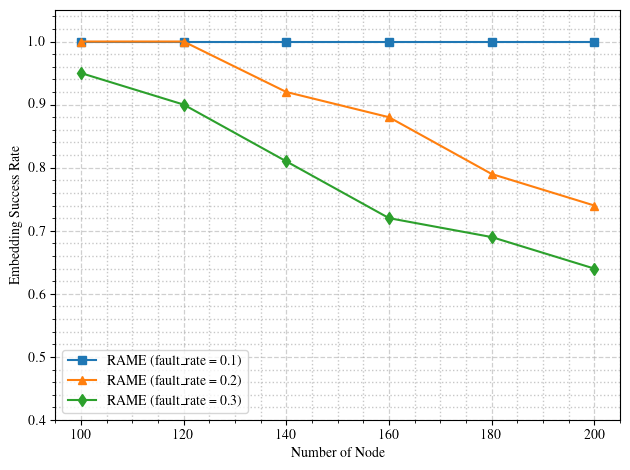
\includegraphics[ width=\linewidth]{Fig_MaiDinhCong/number of node embedding success rate.png}
% 		\subcaption{}
% 	\end{minipage}
% 	\caption{Embedding success rate for problems of size 200 as the fault rate increases, evaluated under different graph densities: 0.5, 0.6, and 0.7. The right figure show embedding success rate as the problem size increases from 100 to 200, with a fixed graph density of 0.5. Results are evaluated under varying fault rates: 0.1, 0.2, and 0.3.}
% 	\label{fig:average and percent}
% \end{figure}

% Figure~\ref{fig:success rate} presents the embedding success rate for problem instances consisting of 200 logical qubits under varying fault rates and graph densities. The success rate is defined as the ratio of logical qubits that are successfully embedded onto the hardware to the total number of logical qubits (i.e., $200$ in this case). As expected, higher edge densities in the logical graph reduce the success rate of minor embedding. This is because denser graphs require more physical qubits and couplers to preserve the necessary logical connectivity during embedding. For instance, at a fault rate of 15\%, the success rate decreases from 0.94 for a graph with density 0.5, to 0.90 for density 0.6, and further to 0.82 for density 0.7. Additionally, increasing the fault rate significantly degrades embedding feasibility. As more qubits become unavailable due to hardware faults, the available physical resources become insufficient to support large chains or maintain inter-chain connectivity. For example, with a fault rate of 5\%, our proposed algorithm is able to embed all 200 logical qubits. However, at a fault rate of 30\%, the success rate drops to 0.64 for a density of 0.5, reflecting the severe impact of qubit failures on embedding capacity. These results highlight the importance of fault-aware embedding strategies in maintaining solution feasibility under realistic hardware constraints. Our proposed method demonstrates robust performance across a range of densities and fault scenarios, outperforming traditional approaches in degraded environments.

% Figure~\ref{fig:success_rate_problem_increase} illustrates the embedding success rate as a function of problem size, with the number of logical qubits increasing from 100 to 200. All problem instances are generated with a fixed graph density of 0.5, and results are reported under fault rates of 10\%, 20\%, and 30\%. The results indicate a clear trend: as the problem size increases, the probability of successful embedding decreases. This decline is primarily due to the increased demand for physical resources—larger logical problems require more qubits and couplers to preserve the connectivity of the original problem graph. Under limited hardware capacity, particularly in the presence of faults, this demand may exceed the available resources. For instance, with a fault rate of 30\%, the embedding success rate is 1.0 when the problem consists of 100 logical qubits, indicating that all instances are successfully embedded. However, as the problem size increases to 200 qubits, the success rate drops to 0.65. This result underscores the scalability challenge of minor embedding and highlights the importance of fault-aware embedding strategies to maximize success under increasing hardware constraints.
% \bibliography{Fig_MaiDinhCong/ref}  
% \end{document}